\section{Introduction}
\subsection{Background}
Carbonic anhydrase (CA) catalyzes the interconversion of carbon dioxide and carbonic acid/bicarbonate as follows:
\begin{align}\label{eqn:ca_reaction}
\ce{CO_2 + H_2O
<=>[\ce{CA}]
H_2CO_3}
\end{align}
Lindskog and Coleman showed the catalytic activity of carbonic anhydrase to be most efficient at neutral pH \cite{bib:ca_ph_dependence}; therefore, while investigating CA activity, maintaining neutral pH with a buffer is a good idea. As Figure \ref{fig:ca_active_site} illustrates, the CA active site contains a \ce{Zn^2+} cofactor (denoted as CA$\cdot$Zn), upon which the enzyme relies for its catalytic activity. The zinc ion can be stripped from the enzyme using a Lewis base ligand, which donates electrons to the ion to form a covalent bond. The ligand being studied in this experiment is 2,6-pyridinecarboxylate, commonly called dipicolinate (or dipic). Figure \ref{fig:dipic} shows the structure of dipic. In this experiment, the rate of zinc removal by dipic will be measured.

\begin{figure}[h]
  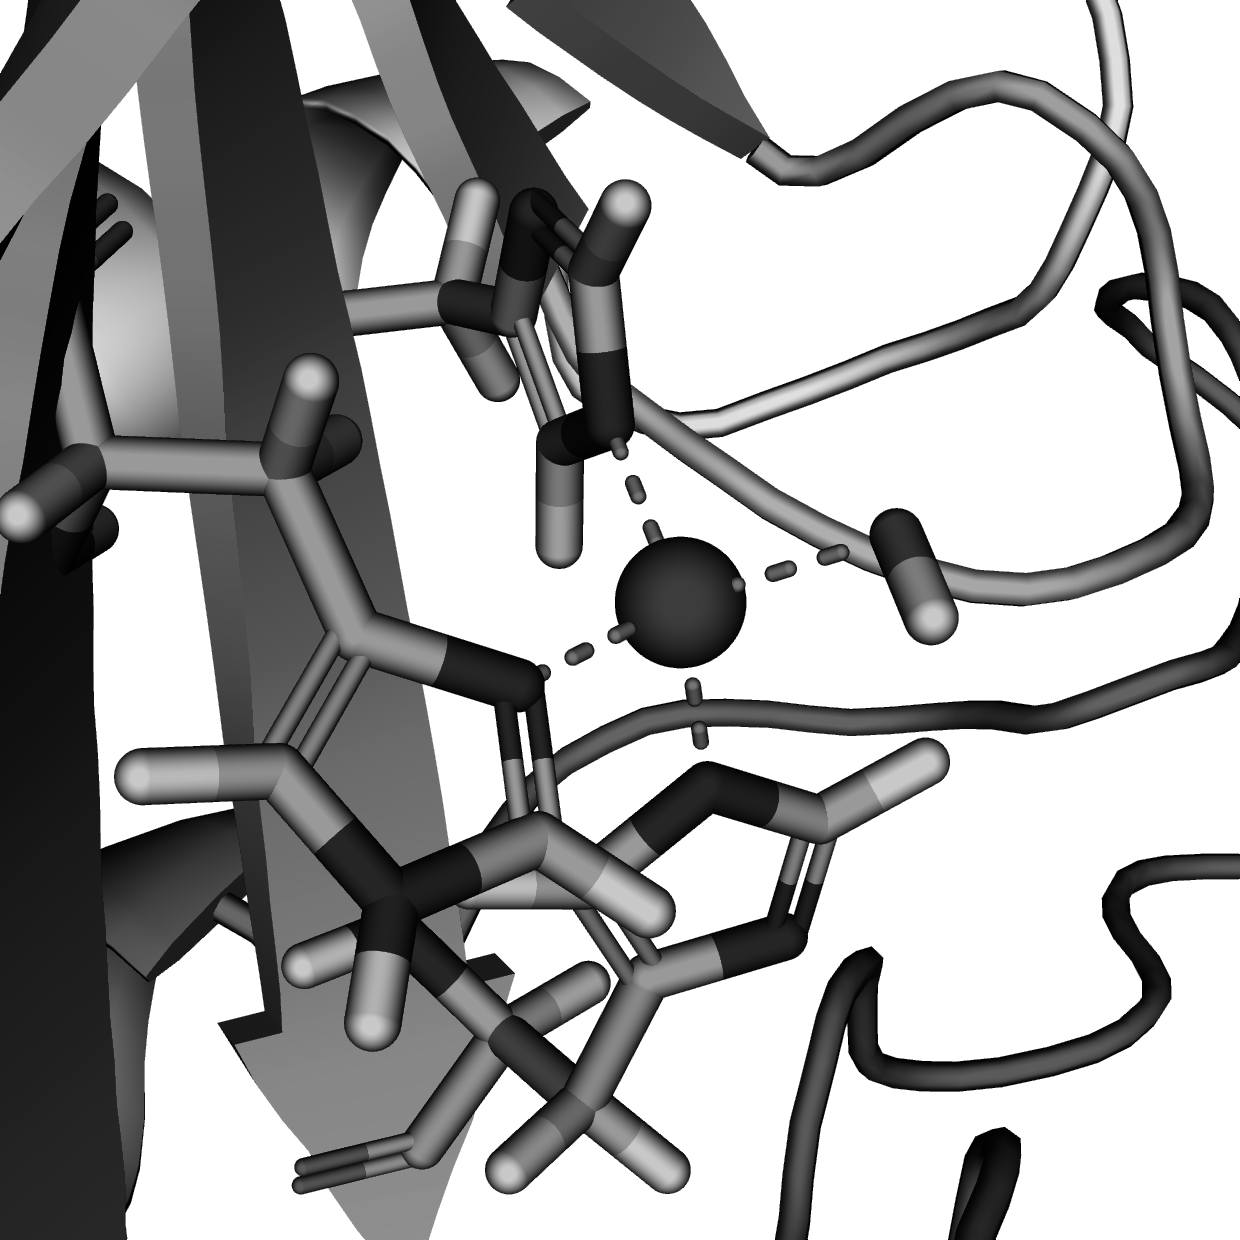
\includegraphics[width=.9\textwidth]{./Figures/Carbonic_anhydrase_1CA2_active_site_gray.png}\\
  \caption{\ce{Zn^2+} cofactor in the active site of human carbonic anhydrase II\cite{bib:pdb_carbonicanhydrase}}\label{fig:ca_active_site}
\end{figure}

\begin{figure}[h]
  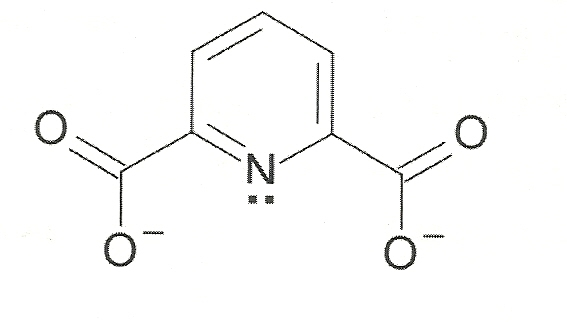
\includegraphics[scale=0.5]{./Figures/dipic.jpg}\\
  \caption{Structure of 2,6-pyridinecarboxylate (dipic)\cite{bib:lab_manual}}\label{fig:dipic}
\end{figure}

\subsection{Mechanism}
When $[dipic] >> [CA]$, that is, when $\frac{[dipic]}{[CA]} \ge 25$, the removal of zinc is pseudo-first-order with respect to CA$\cdot$Zn because the concentration of dipic, denoted as L, does not change appreciably. Thus the formation of the inactive enzyme, apoCA, can be modeled using the following rate equation:
\begin{equation}\label{eqn:apoCA_kobs}
\frac{d[\text{apoCA}]}{dt}=k_{obs}[\text{CA$\cdot$Zn}]
\end{equation}
The pseudo-first-order rate constant, $k_{obs}$, increases as [L] increases, but levels off at sufficiently high concentrations of L. Biochemists will recognize behavior similar to Michaelis-Menten enzyme kinetics in which the enzyme, CA$\cdot$Zn, and the substrate, L, reversibly form a CA$\cdot$Zn$\cdot$L complex with association constant $K_{EML}$ (EML stands for Enzyme-Metal-Ligand):
\begin{align}\label{eqn:KEML_reaction}
\ce{CA$\cdot$Zn + L
<=>[\ce{K_{EML}}]
CA$\cdot$Zn$\cdot$L}
\end{align}
This can be modeled as follows:
\begin{equation}\label{eqn:KEML_expression}
K_{EML}=\frac{\text{[CA$\cdot$Zn$\cdot$L]}}{\text{[CA$\cdot$Zn][L]}}
\end{equation}

CA$\cdot$Zn$\cdot$L can either revert back to the original species or irreversibly convert to the inactive form of the enzyme, apoCA, and the covalently bound zinc-dipic molecule, ZnL:
\begin{align}\label{eqn:kd_reaction}
\ce{CA$\cdot$Zn$\cdot$L
->[\ce{k_{d}}]
apoCA + ZnL}
\end{align}
This yields the following differential rate law:
\begin{equation}\label{eqn:kd_expression}
\frac{d[\text{apoCA}]}{dt}=k_{d}[\text{CA$\cdot$Zn$\cdot$L}]
\end{equation}
Note the difference in assumptions between this reaction and the Michaelis-Menten model; M-M kinetics assumes the enzyme is reformed and that only the substrate is modified, while Reaction \eqref{eqn:kd_reaction} shows that both the substrate and the enzyme are permanently modified. Recall that $\text{[L]} >> \text{[CA$\cdot$Zn]}$, so [L] can be treated as a constant, $\text{[L]}_0$, which is substituted into a rearranged form of Equation \eqref{eqn:KEML_expression},
\begin{equation}\label{eqn:KEML_expression_constant_L}
\text{[CA$\cdot$Zn$\cdot$L]}=K_{EML}\text{[CA$\cdot$Zn][L]}_0
\end{equation}

Carbonic anhydrase can exist in one of three forms: the metalloenzyme CA$\cdot$Zn, the enzyme-metal-ligand complex CA$\cdot$Zn$\cdot$L, or the inactivated enzyme apoCA. Initially, all CA is tied up in the metalloenzyme, and none exists as CA$\cdot$Zn$\cdot$L or apoCA. As the activated form of the enzyme gets bound to L and then inactivated,
\begin{equation}\label{eqn:CAZnconc}
\text{[CA$\cdot$Zn]}=\text{[CA$\cdot$Zn]}_0 - \text{[apoCA]} - \text{CA$\cdot$Zn$\cdot$L},
\end{equation}
which can be combined with Equation \eqref{eqn:KEML_expression_constant_L} to yield
\begin{equation}\label{eqn:CAZnconc_EMLsub}
\text{[CA$\cdot$Zn]}=\text{[CA$\cdot$Zn]}_0 - \text{[apoCA]} - K_{EML}\text{[CA$\cdot$Zn][L]}_0
\end{equation}
and rearranged as follows:
\begin{equation}\label{eqn:CAZnconc_EMLsub_rearrange}
\text{[CA$\cdot$Zn]}=\frac{\text{[CA$\cdot$Zn]}_0 - \text{[apoCA]}}{1+K_{EML}\text{[L]}_0}
\end{equation}

Equations \eqref{eqn:kd_expression} and \eqref{eqn:KEML_expression_constant_L} can be combined to give
\begin{equation}\label{eqn:rate_apoCA_formation_wrt_kdkeml}
\frac{d[\text{apoCA}]}{dt}=k_{d}K_{EML}\text{[CA$\cdot$Zn][L]}_0
\end{equation}
Therefore, in a solution containing dipic in large excess, the rate of apoCA formation is first-order with respect to CA$\cdot$Zn. Combining equations \eqref{eqn:rate_apoCA_formation_wrt_kdkeml} and \eqref{eqn:CAZnconc_EMLsub_rearrange} yields
\begin{equation}\label{eqn:preintegration}
\frac{d[\text{apoCA}]}{dt}=k_{d}K_{EML}\text{[L]}_0\frac{\text{[CA$\cdot$Zn]}_0 - \text{[apoCA]}}{1+K_{EML}\text{[L]}_0}
\end{equation}
Rearranging and integrating,
\begin{align}\label{eqn:kdkeml_integral}
\begin{split}
\int_{[apoCA]_0}^{[apoCA]_t} \frac{d[\text{apoCA}]}{\text{[CA$\cdot$Zn]}_0 - \text{[apoCA]}_t} &= \int_0^t \frac{k_{d}K_{EML}\text{[L]}_0}{1+K_{EML}\text{[L]}_0}dt \\
&= \frac{k_{d}K_{EML}\text{[L]}_0}{1+K_{EML}\text{[L]}_0}t
\end{split}
\end{align}
The left side must be integrated using u-substitution:
\begin{equation*}
u=\text{[CA$\cdot$Zn]}_0 - \text{[apoCA]}_t
\end{equation*}
\begin{equation*}
du=-d[\text{apoCA}]
\end{equation*}
To change the integral boundaries,
\begin{equation*}
u(t=0)=\text{[CA$\cdot$Zn]}_0\text{, since no inactivated enzyme has been formed}
\end{equation*}
\begin{equation*}
u(t=t)=\text{[CA$\cdot$Zn]}_0 - \text{[apoCA]}_t
\end{equation*}
Therefore,
\begin{align}\label{eqn:long_integral}
\begin{split}
\int_{[apoCA]_0}^{[apoCA]_t} \frac{d[\text{apoCA}]}{\text{[CA$\cdot$Zn]}_0 - \text{[apoCA]}_t}
&=
-\int_{\text{[CA$\cdot$Zn]}_0}^{\text{[CA$\cdot$Zn]}_0 - \text{[apoCA]}_t} \frac{du}{u} \\
&=
-ln(u) \Big|_{\text{[CA$\cdot$Zn]}_0}^{\text{[CA$\cdot$Zn]}_0 - \text{[apoCA]}_t} \\
&= -ln \left( \frac{\text{[CA$\cdot$Zn]}_0 - \text{[apoCA]}}{\text{[CA$\cdot$Zn]}_0} \right)
\end{split}
\end{align}

Combining the evaluated integrals from equations \eqref{eqn:long_integral} and \eqref{eqn:kdkeml_integral} yields
\begin{equation}\label{eqn:integrated_rate_law}
ln \left( \frac{\text{[CA$\cdot$Zn]}_0 - \text{[apoCA]}}{\text{[CA$\cdot$Zn]}_0} \right)
=
-\frac{k_{d}K_{EML}\text{[L]}_0}{1+K_{EML}\text{[L]}_0}t
\end{equation}
Assuming [CA$\cdot$Zn$\cdot$L] is always negligible, $\frac{\text{[CA$\cdot$Zn]}_0 - \text{[apoCA]}}{\text{[CA$\cdot$Zn]}_0}$ is simply the fraction of CA$\cdot$Zn remaining after reaction time $t$ and can be referred to as $F_\text{CA$\cdot$Zn}$:
\begin{equation}\label{eqn:integrated_rate_law_frac}
ln \left( F_\text{CA$\cdot$Zn} \right)
=
-\frac{k_{d}K_{EML}\text{[L]}_0}{1+K_{EML}\text{[L]}_0}t
\end{equation}
Since $-\frac{k_{d}K_{EML}\text{[L]}_0}{1+K_{EML}\text{[L]}_0}$ is a constant for a given concentration of dipic, Equation \eqref{eqn:integrated_rate_law_frac} exhibits linear behavior over time while the solution contains active enzyme. Therefore, a linear least squares regression procedure can be performed for measurements of $ln \left( F_\text{CA$\cdot$Zn} \right)$ over time (until those measurements level off, which indicates that all the enzyme is used up), and the slope, denoted $-k_{obs}$, will be
\begin{equation}\label{eqn:kobs_slope}
-k_{obs}
=
-\frac{k_{d}K_{EML}\text{[L]}_0}{1+K_{EML}\text{[L]}_0}
\end{equation}

Taking the reciprocal of Equation \eqref{eqn:kobs_slope} yields
\begin{equation}\label{eqn:kobs_slope_reciprocal}
\begin{split}
\frac{1}{k_{obs}}
&=
\frac{1+K_{EML}\text{[L]}_0}{k_{d}K_{EML}\text{[L]}_0} \\
&= \frac{1}{k_{d}K_{EML}\text{[L]}_0} + \frac{K_{EML}\text{[L]}_0}{k_{d}K_{EML}\text{[L]}_0} \\
&= \frac{1}{k_{d}K_{EML}} \times \frac{1}{\text{[L]}_0} + \frac{1}{k_{d}}
\end{split}
\end{equation}
Again, a linear relationship is observed; measuring $k_{obs}$ at several different dipic concentrations enables one to perform a least squares regression procedure on $\frac{1}{k_{obs}}$ versus $\frac{1}{\text{[L]}_0}$ to determine the slope, $m=\frac{1}{k_{d}K_{EML}}$, and intercept, $b=\frac{1}{k_{d}}$. $k_d$ and $K_{EML}$ are thus calculated as follows:
\begin{equation}\label{eqn:calculating_kd}
k_d=\frac{1}{b}
\end{equation}
\begin{equation}\label{eqn:calculating_keml}
K_{EML}=\frac{b}{m}
\end{equation}

Deriving $k_d$ and $K_{EML}$ using Equation \eqref{eqn:kobs_slope_reciprocal} requires varying the dipic concentration while holding constant the concentration of carbonic anhydrase. As stated in the procedure, a certain volume, $v_L$, of dipic with a given concentration, $\text{[L]}_{stock}$, is added to a solution of carbonic anhydrase and phosphate buffer in order to dilute the dipic to a desired concentration, $\text{[L]}_0$. The final volume of solution is $v_{soln}$. In order to calculate the needed dipic volume,
\begin{equation}\label{eqn:dipic_dilution}
v_L=\frac{v_{soln} \times \text{[L]}_0}{\text{[L]}_{stock}}
\end{equation}
The amount of phosphate buffer, $v_{buff}$, needed to bring the solution to $v_{soln}$, is simply
\begin{equation}\label{eqn:buff_volume}
v_{buff}=v_{soln}-v_{CA}-v_L
\end{equation}
where $v_{CA}$ is the original carbonic anhydrase solution volume.

\subsection{Rate Measurements}
While Equation \eqref{eqn:kobs_slope} seems to imply that the determination of $k_{obs}$ requires knowing [CA$\cdot$Zn] or [apoCA] at any point in time, in reality a plot of $f(t)$ vs $t$, where $t$ refers to CA/dipic reaction time and $f(t)$ is proportional to $F_\text{CA$\cdot$Zn}$, will still exhibit the same slope $-k_{obs}$. The Michaelis-Menten kinetics model states that, for sufficiently large substrate concentrations, the enzyme is fully saturated and the reaction velocity asymptotically approaches a constant rate,
\begin{equation}\label{eqn:vmax}
V_{max}=k_{cat}\text{[CA$\cdot$Zn]}\text{,} 
\end{equation}
where $k_{cat}$ (the ``turnover number'') is the amount of substrate that a single saturated enzyme molecule can convert to produce in a given unit of time \cite{bib:lehninger_mm}. Thus for sufficiently large concentrations of substrate, the enzyme catalytic activity fulfills the requirement of proportionality to $F_\text{CA$\cdot$Zn}$. Ideally, the determination of the enzymatic activity from $V_{max}$, that is, taking an enzyme assay, can be done using a substrate which is cheap, readily available, and easily measurable. As Figure \ref{fig:pnpa_reaction} shows, carbonic anhydrase happens to hydrolyze para-nitrophenyl acetate (pNPA) to form para-nitrophenol and acetic acid:
\begin{figure}[h]
  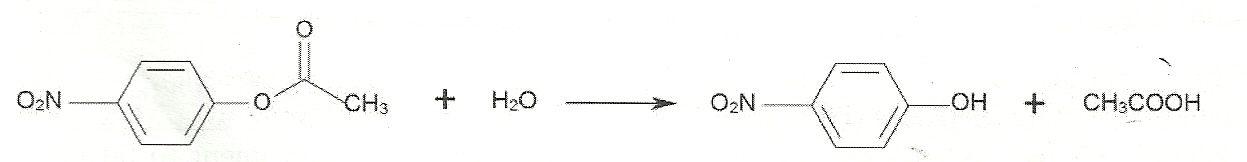
\includegraphics[width=.9\textwidth]{./Figures/pnpa_hydrolysis.jpg}\\
  \caption{Carbonic anhydrase-catalyzed hydrolysis of para-nitrophenyl acetate (pNPA) to para-nitrophenol and acetic acid \cite{bib:lab_manual}}\label{fig:pnpa_reaction}
\end{figure}

Para-nitrophenol absorbs strongly at 348nm. Recall that Beer's law states
\begin{equation}\label{eqn:beers_law}
A=\epsilon b c
\end{equation}
where $A$ is the measured absorbance at a particular wavelength, $\epsilon$ is the molar absorptivity, $b$ is the measurement path length, and $c$ is the concentration \cite{bib:quantitative_chem_anal_beer_law}. Since $b$ and $\epsilon$ stay constant, $A$ is dependent only on $c$. The concentration varies with time, therefore the change in absorbance under enzyme-catalyzed conditions, $\left(\frac{dA}{dt}\right)_{cat}$, is proportional to the para-nitrophenol formation velocity, which, as \eqref{eqn:vmax} demonstrates, is itself proportional to the amount of active carbonic anhydrase in solution. Because the reaction occurs to a nontrivial extent without enzymatic catalysis, a baseline correction is needed, $(\frac{dA}{dt})_{uncat}$, which can be obtained either from a solution containing only pNPA or a mixture of pNPA and apoCA (that is, an assay taken after sufficient time has passed to inactivate all extant carbonic anhydrase). In this experiment, $(\frac{dA}{dt})_{uncat}$ was determined from the solution of pNPA with no enzyme added. Thus, Equation \eqref{eqn:integrated_rate_law_frac} can be implemented using
\begin{equation}\label{eqn:baseline_correction}
ln \left(\frac{dA}{dt}\right)_{cat} = ln \left( \frac{ \left (\frac{dA}{dt}\right)_{t} }{ \left (\frac{dA}{dt}\right)_{uncat} } \right)
\end{equation} 
(note: this also fulfills the logarithm function's unitless requirement.)